\documentclass[../main.tex]{subfiles}
\graphicspath{{\subfix{../../images/}}}

\begin{document}

The von neumann architecture specifies a generic structure for CPUs and microprocessors to follow when they are designed. It dictates that the data used to store programs and the data used by the program (tempoary values, variables in memory) should co-exist in the same memory.

The following is a diagram of the von neumann architecture:

\begin{figure}[H]
    \centering
    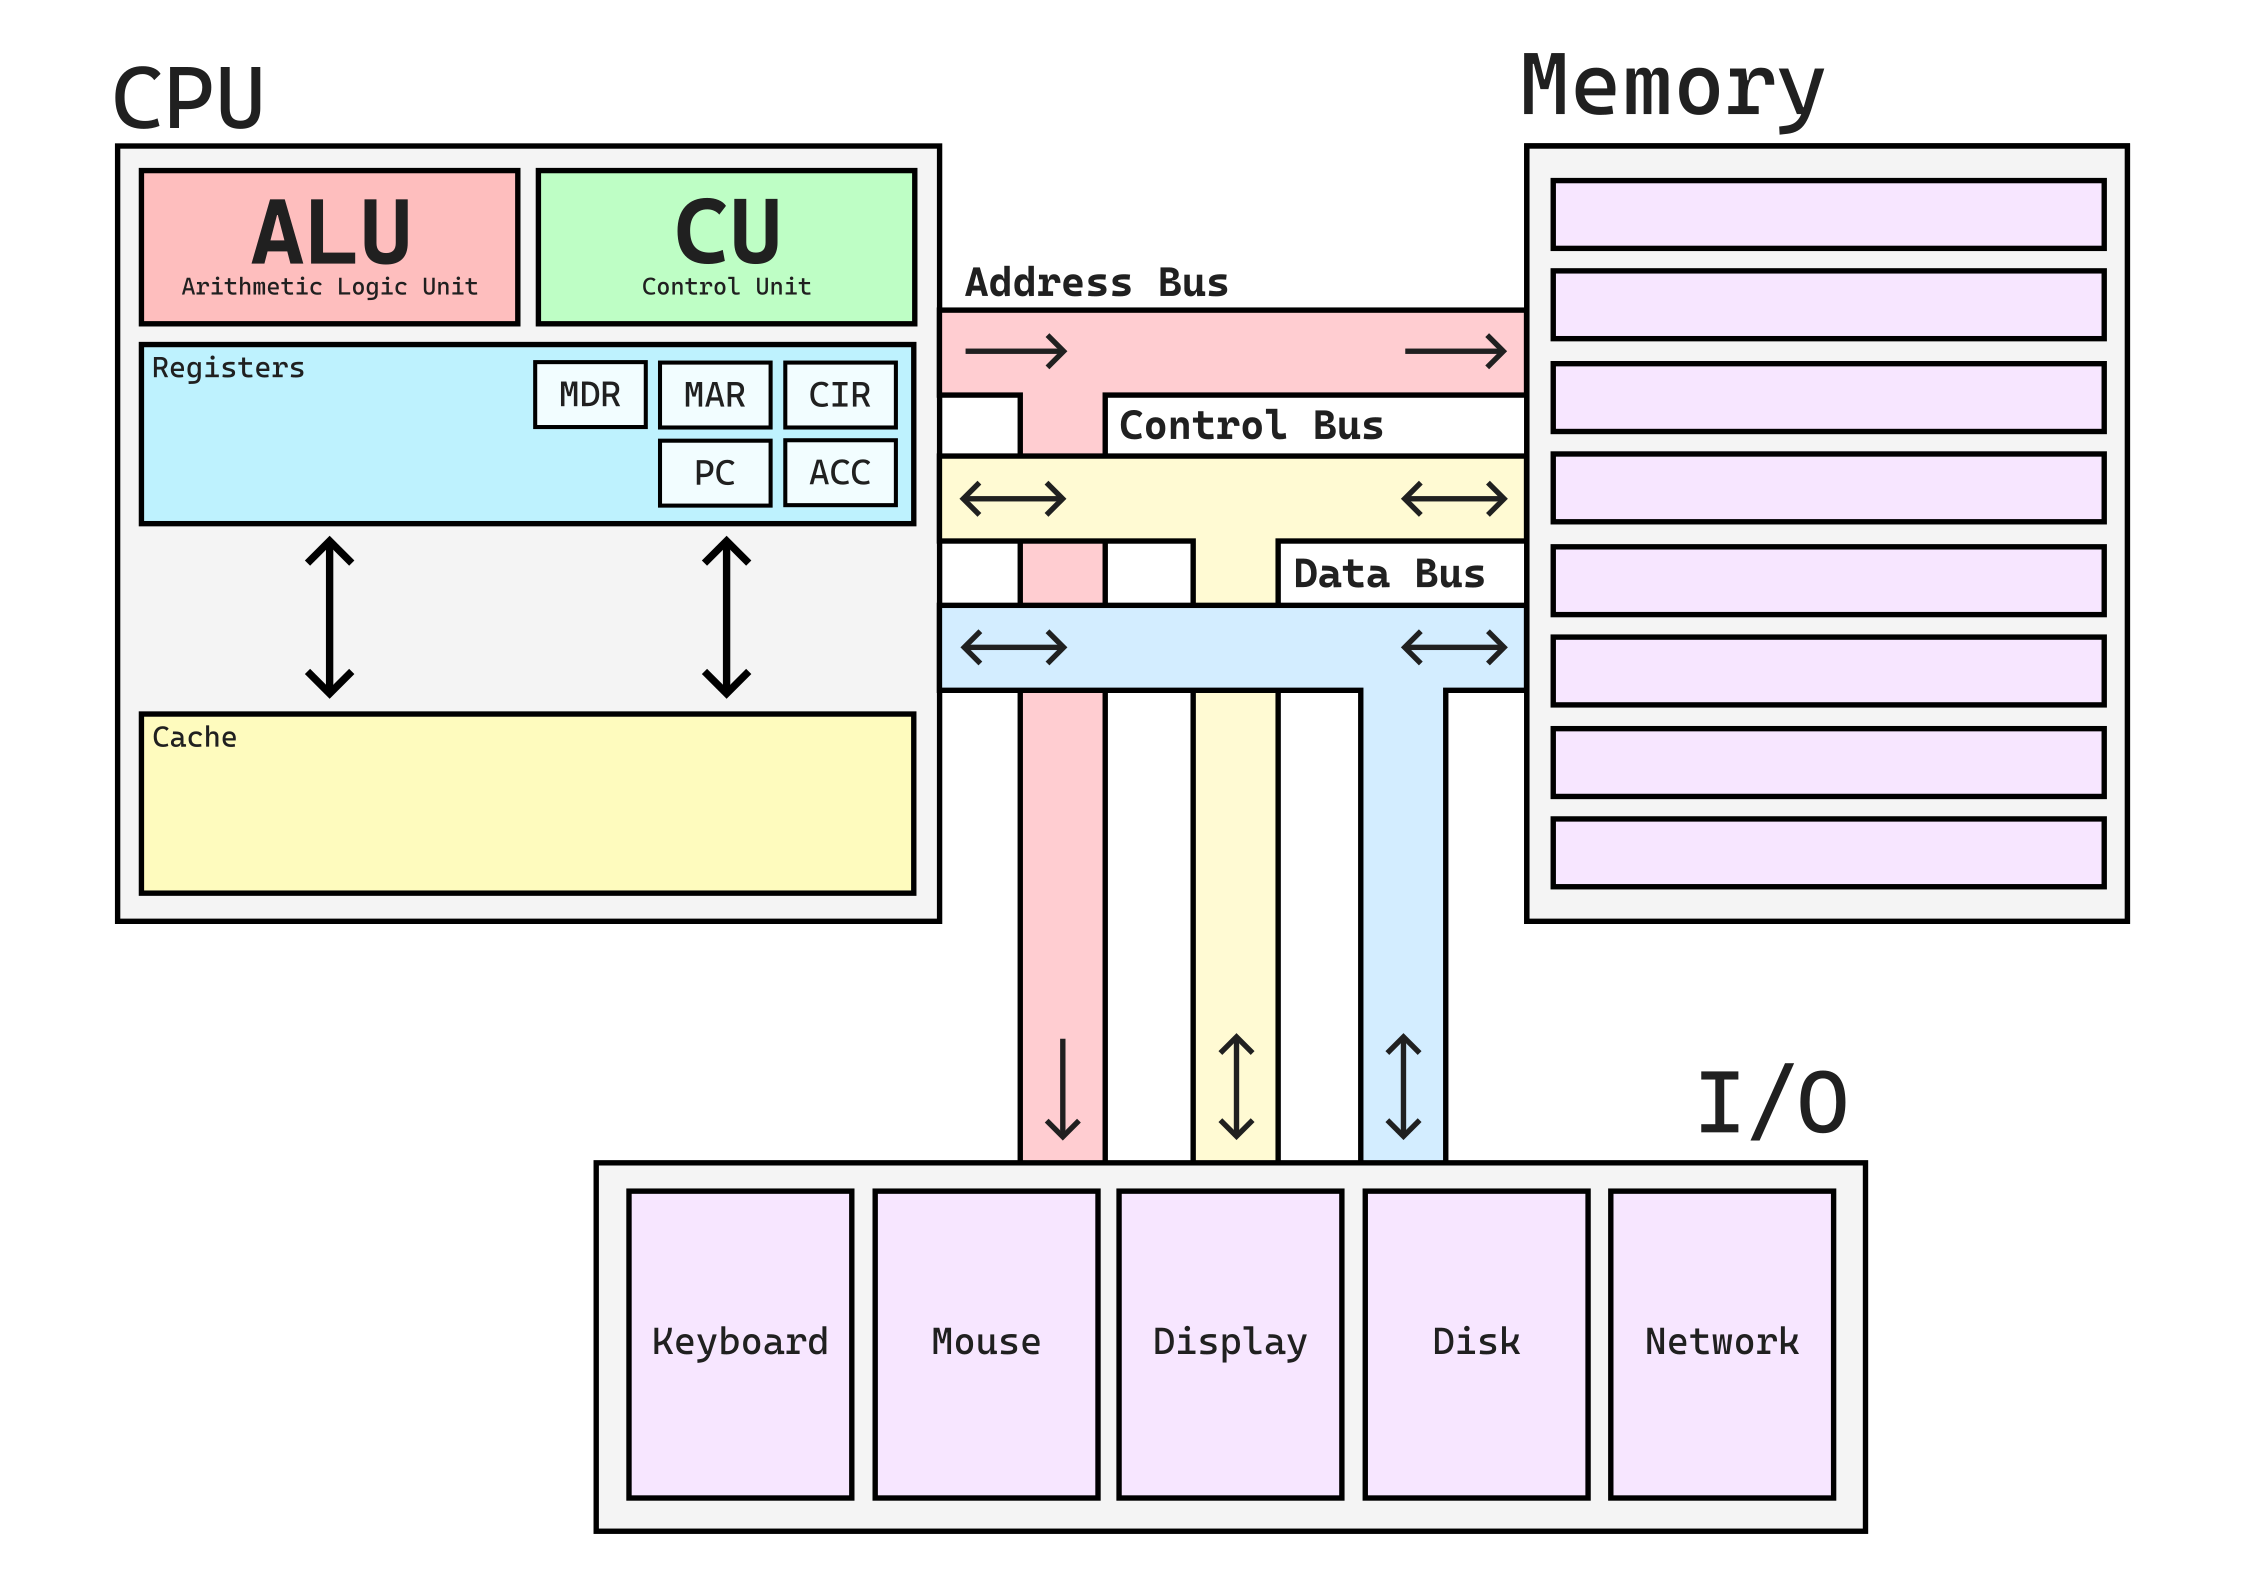
\includegraphics[width=0.85\textwidth]{vonneumann.png}
    \caption{A bird's eye view of the von neumann architecture.}
    \label{fig:vonneumann}
\end{figure}

\subsection{The CPU}
\label{3:sec:cpu}

The CPU or the Central Processing Unit is the brains of your computer. It carries out all the instructions ever passed through your CPU, and is the center of your computer's activity. Modern CPUs have the ability to do many things at once, like playing music while doing word processing\footnote{A very, very, very oversimplified example.}

CPUs look like this:

\begin{figure}[H]
    \centering
    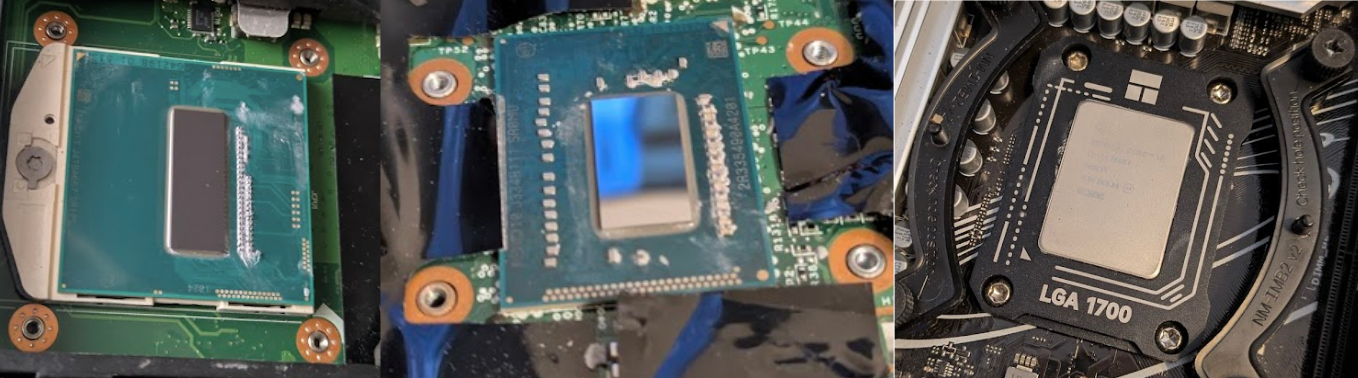
\includegraphics[width=0.85\textwidth]{cpus.png}
    \caption{An Laptop CPU in a socket, an Intel Core i7-4712MQ, a Laptop CPU directly soldered on the motherboard, an Intel Core i7-3520M, and a desktop Intel Core i7-14700KF.}
    \label{fig:cpus}
\end{figure}

\emph{Extra: The shiny part of the CPU is called the die. The die is filled with extremely dense transistors which are all semi-conductive. The die actually does the processing. For those who wonder, no, you cannot see the individual transistors and registers on the CPU; they are so incredibly small and the parts of the CPU are so incredibly small it is impossible to reverse-engineer its architecture; even with microscopes}.

Inside the CPU, there are many important components that are critical to its function. Figure \ref{fig:vonneumann} and \ref{fig:cpu_vonneumann} shows this. Each section that follows explains each part of the diagram. For information on Memory and I/O (or IO), See section \ref{3:sec:ram} and \ref{3:sec:input_and_output_devices} respectively.

\begin{figure}[H]
    \centering
    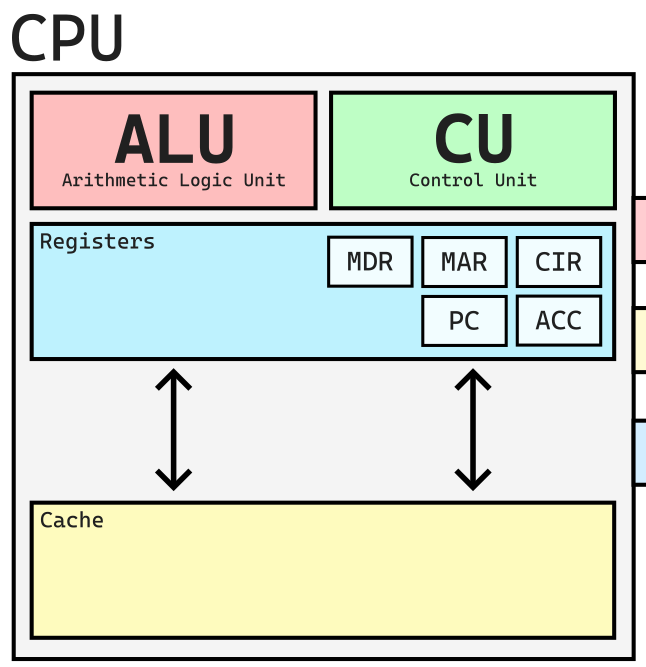
\includegraphics[width=0.4\textwidth]{cpu_vonneumann.png}
    \caption{The CPU on the inside}
    \label{fig:cpu_vonneumann}
\end{figure}

\subsection{The CU, ALU and Registers}

The Control Unit, or CU is like the boss of your CPU. All operations that involve sending data to and from memory or interacting with I/O devices like the mouse and keyboard (refer to figure \ref{fig:vonneumann}) is done by the control unit. It is also responsible for decoding instructions for the CPU to execute.

The ALU or the Arithmetic Logic Unit is responsible for performing all mathematical and logical operations, like addition, multiplication and so on, along with AND, OR, NOT, etc. For more information on logical operations, see section \ref{10:sec:logic_gates}.

Registers, like RAM is for fast data storage. The main difference between registers and main memory is that registers are built into the CPU itself. Registers store very little data, typically only 64 bit integers; but are much, much faster than main memory. They also typically serve special purposes. In the diagram, there are 5 important registers that are important for CPU operation.

\begin{itemize}
    \item \textbf{The Program Counter (PC):} Program 
\end{itemize}

\subsection{Cache}

\subsection{Buses}

\subsection{The Fetch-Decode-Execute Cycle}

\subsection{The Clock Speed}

\subsection{Increasing CPU speed}

\subsection{Cores}

Cores are like Sub-CPUs in each CPU. Each CPU shown in figure \ref{fig:cpus} has more than 1 core. Each of them can carry out tasks independently of each other; despite how they can communicate together. For those who have already read this whole section, each core can carry out its own fetch-decode-execute cycle.

\begin{figure}[H]
    \centering
    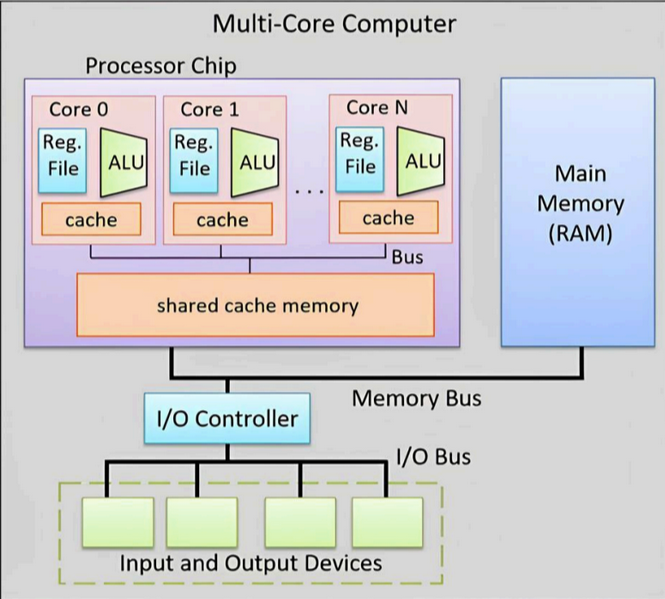
\includegraphics[width=0.7\textwidth]{cores.png}
    \caption{A diagram showing what cores look like in a CPU.}
    \label{fig:cores}
\end{figure}


\end{document}
